\begin{figure}[t]
\centering
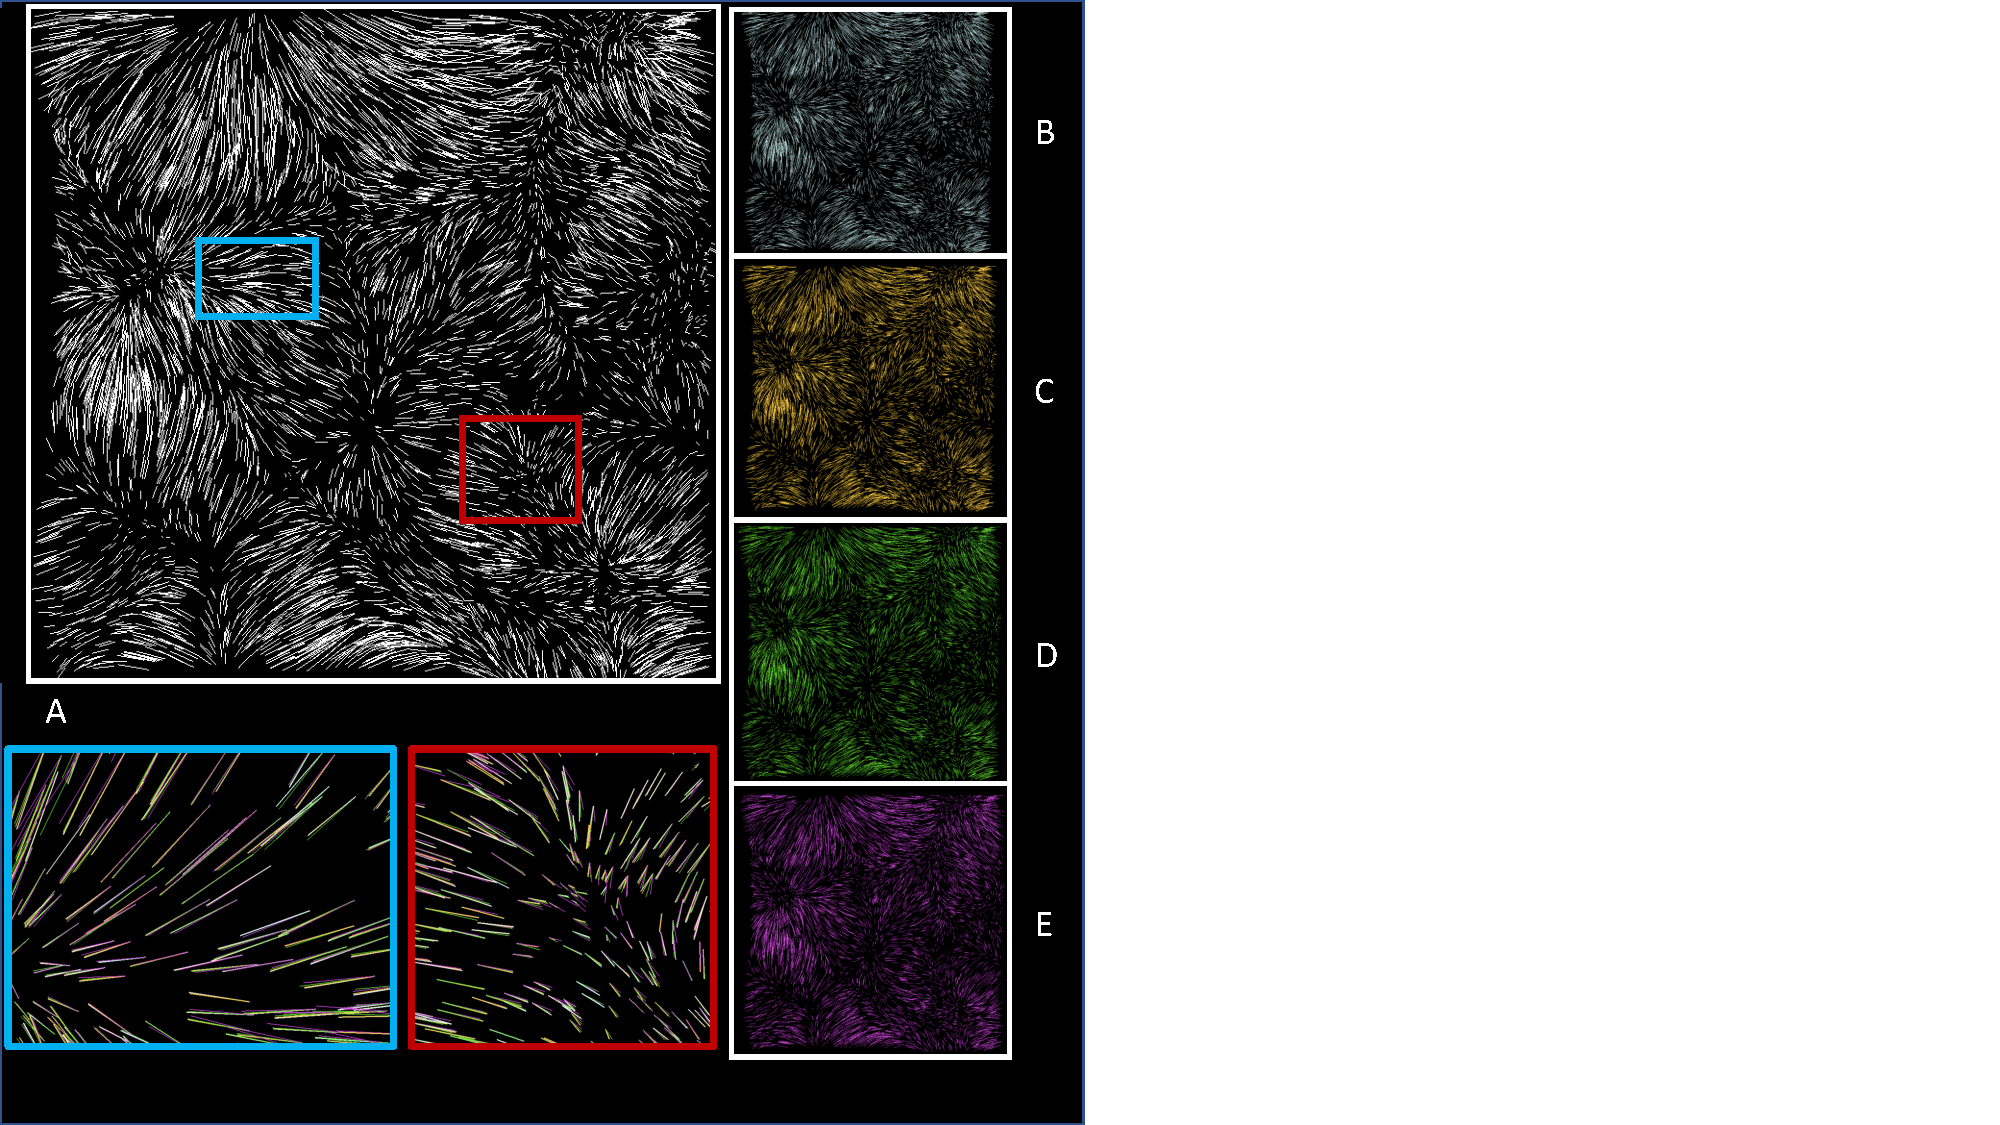
\includegraphics[width=0.87\linewidth, trim={0cm 1cm 15.5cm 0cm}, clip]{images/Nyx_Vis.pdf}
\vspace{-3mm}
\caption{A qualitative comparison of pathlets reconstructed over one interval for the Nyx data (\textbf{Interval = 25} case). For each configuration we specify \textbf{DS-1} and \textbf{PHE-1} as (Bytes, Cell Side\%). Image A (white) is the ground truth, B~(light-blue) is Eulerian~(227MB; 2.29\%), C~(yellow) is Lagrangian 1:1~(232MB; 11.61\%), D~(green) is Lagrangian 1:8~(27MB; 37.27\%), E~(pink) is Lagrangian 1:27~(8MB; 72.727\%).} 
\label{fig:nyx_vis}
\vspace{-5mm}
\end{figure}
